% Final report, Machine Learning group project, Bachelor in Applied Mathematics, IE University.
% Follows the structure of the submitted "Project Proposal and Progress Report".
% Compile: tectonic main.tex   (figures from ./figures and ../progress/figures)
\documentclass[11pt]{article}
\usepackage[margin=1in]{geometry}
\usepackage[T1]{fontenc}
\usepackage[utf8]{inputenc}
\usepackage{lmodern}
\usepackage{microtype}
\usepackage{graphicx}
\usepackage{booktabs}
\usepackage{amsmath,amssymb}
\usepackage{enumitem}
\usepackage{xcolor}
\usepackage{fancyhdr}
\usepackage[hidelinks]{hyperref}
\usepackage{caption}
\usepackage{tabularx}
\usepackage{float}
\usepackage[section]{placeins}
\usepackage{titlesec}

\captionsetup{font=small,labelfont=bf,labelsep=period,skip=4pt}
\setlist{topsep=2pt,itemsep=1pt,parsep=0pt}
\graphicspath{{figures/}{../progress/figures/}}
\pagestyle{fancy}\fancyhf{}
\lhead{\small Street-Level Country Classification}\rhead{\small Bachelor in Applied Mathematics}
\cfoot{\thepage}
\setlength{\headheight}{14pt}
\titlespacing*{\section}{0pt}{10pt plus 2pt minus 2pt}{5pt plus 1pt}
\titlespacing*{\subsection}{0pt}{8pt plus 2pt minus 2pt}{3pt plus 1pt}
\titlespacing*{\subsubsection}{0pt}{6pt plus 2pt minus 1pt}{2pt plus 1pt}
\setlength{\textfloatsep}{8pt plus 2pt minus 2pt}
\setlength{\floatsep}{6pt plus 2pt minus 2pt}
\setlength{\intextsep}{6pt plus 2pt minus 2pt}
\renewcommand{\topfraction}{0.9}\renewcommand{\bottomfraction}{0.8}
\renewcommand{\textfraction}{0.1}\renewcommand{\floatpagefraction}{0.8}
\setcounter{topnumber}{3}\setcounter{bottomnumber}{2}\setcounter{totalnumber}{4}
\AtBeginDocument{\setlength{\abovedisplayskip}{4pt plus 2pt minus 2pt}\setlength{\belowdisplayskip}{4pt plus 2pt minus 2pt}}
\raggedbottom
\interlinepenalty=10000
\predisplaypenalty=10000
\postdisplaypenalty=10000
\widowpenalty=10000
\clubpenalty=10000
\displaywidowpenalty=10000
\newcommand{\tsh}{test\textsubscript{shared}}
\newcommand{\vsh}{val\textsubscript{shared}}
\newcommand{\pp}{\,pp}

\begin{document}
\begin{titlepage}
\centering
\vspace*{5cm}
{\large\bfseries Final Report\par}\vspace{1cm}
{\LARGE\bfseries Learning Where: Country Classification from\\[4pt] Crowd-Sourced Street-Level Imagery\par}
\vspace{1cm}
{\large Machine Learning -- Group Project\par}\vspace{4pt}
Bachelor in Applied Mathematics\\ IE University
\vfill
{\bfseries Team members}\\[4pt] Kwanhyung Kim\\ Guillermo Gonzalez\\[1cm]
{\bfseries Professor}\\[4pt] Nacho Molina Clemente
\vfill
Fall 2026--2027
\end{titlepage}

\section*{Abstract}
Can a convolutional neural network trained on crowd-sourced street-level imagery recognise countries in
photos by people it has never seen, or does it partly recognise the people? On 32 countries of
OpenStreetView-5M, we split photographers rather than images between training and test, and compare
accuracy on unseen photographers with accuracy on new trips of photographers seen in training. An
end-to-end fine-tuned ResNet-18 reaches 31.9\% balanced accuracy on unseen photographers (chance 3.1\%),
but 5.2\pp\ more on familiar ones. This gap is absent from frozen ImageNet features, rises with the number
of a photographer's images in training, and is largely explained by retrieving the same photographer's
other photos; it is also local, about 8\pp\ within 25\,km of the photographer's training trips and
none beyond 100\,km. Removing the camera
fingerprint during training (blanking the bonnet band, compression and colour jitter) shrinks the gap to
3.1\pp\ but costs 3.6\pp\ on unseen photographers, because the same pixels also show the road. The
network learns countries, but part of its accuracy on familiar photographers comes from recognising where
and with what camera they drive.

\section{Introduction}
\subsection{Research question}
To what extent can a convolutional neural network (CNN) trained end-to-end on crowd-sourced
street-level imagery (OpenStreetView-5M) learn country-discriminative visual features that generalise
beyond the photographers seen during training?

\subsection{Motivation}
GeoGuessr is an online geography game that drops players into a random street-view location and
challenges them to guess where it is (\emph{GeoGuessr}). As travel enthusiasts who grew up as
third-culture individuals, we have always been intrigued by different countries, and became interested in
how neural networks can identify trends in dash-camera images from across the world. Crowd-sourced data
raise a question that benchmark accuracy hides: \emph{whose} images does a model recognise? Photos by
one photographer share the bonnet, windscreen reflections and colour profile of one camera (Luk\'a\v{s}
et al.), so a model can score well by recognising photographers rather than countries, a known form of
shortcut learning (Geirhos et al.; Torralba and Efros; Zech et al.).

\subsection{Related work}
\subsubsection{Image geolocation}
Early work treated geolocation as retrieval: IM2GPS matched a photo to its
nearest geotagged neighbours using hand-crafted colour, texture and scene features (Hays and Efros), and
Doersch et al. mined the small discriminative elements, such as balconies, windows and street signs, that
make one city look different from another, showing that much of a place's identity lies in fine detail.
PlaNet recast the problem as classification over geographic cells with a CNN trained on a very large
collection of geotagged photos (Weyand et al.), and Vo et al. revisited IM2GPS with deep features, finding
that retrieval remains competitive with classification. Recent systems build on large image--text
pretraining: GeoCLIP aligns images with GPS coordinates in a CLIP-style embedding (Vivanco Cepeda et al.),
and PIGEON reaches about 92\% country accuracy on Street View and beats top GeoGuessr players (Haas et al.).

\subsubsection{OpenStreetView-5M}
Astruc et al. built OSV-5M from Mapillary as an open, geographically diverse
benchmark of 5.1M street-level images and compared classification, regression and hybrid models on several
backbones; their best model, a fine-tuned ViT-L/14, reaches 68.0\% country accuracy against 48.9\% for human
players. Their train/test split separates images by location and by sequence but not by photographer, and
the authors note that the same vehicle can appear in both sets. To our knowledge, OSV-5M results are reported on this split only, so the share of accuracy due to recognising photographers is unmeasured.

\subsubsection{Shortcuts and leakage}
Models trained on one dataset exploit its idiosyncrasies (Torralba and
Efros), and deep networks prefer such shortcuts whenever they separate the training data (Geirhos et al.).
The closest analogue to our setting is the pneumonia detector of Zech et al., which partly recognised the
hospital a radiograph came from rather than the disease and generalised worse to other hospitals; a
photographer's camera plays the role of the hospital. The standard remedy is to keep groups of correlated
samples on one side of the split, as grouped cross-validation does (Roberts et al.), and to guard against
information leaking from training to evaluation (Kaufman et al.). Camera identity is known to be recoverable from images, down to the sensor's noise pattern (Luk\'a\v{s} et al.).

\subsubsection{Our contribution}
Rather than maximising accuracy, we measure how much of a country
classifier's accuracy survives for photographers it has never seen, explain where the difference comes
from, and test whether removing camera cues reduces it, using a small model trained on our own hardware.

\subsection{Building on the proposal and progress report}
This report continues our proposal and progress report, whose content is revised up to
Section~\ref{sec:comparison} and extended with the figures our feedback asked for. The progress report
planned an end-to-end $\{$ImageNet, scratch$\}\times\{$standard, fingerprint removal$\}$ design, a wider
probe refit, Grad-CAM and, time permitting, trip aggregation. We train the ImageNet-initialised network
with and without fingerprint removal (Sections~\ref{sec:fpmethod} and~\ref{sec:fp}), add Grad-CAM
(Section~\ref{sec:gradcam}) and trip aggregation (Section~\ref{sec:trips}) and, following the feedback,
analyse which countries are hard and why (Sections~\ref{sec:countries}--\ref{sec:errors}) and the
photographer gap of the new models (Section~\ref{sec:gap}). The from-scratch arm and the probe refit did
not fit our compute (Section~\ref{sec:limits}).

\section{Data}\label{sec:data}
\subsection{Dataset explanation and justification}
We use OpenStreetView-5M, a crowd-sourced Mapillary collection of 4.89M training and 210k test images
from 225 countries (CC BY-SA 4.0) (Astruc et al.). Each image comes with GPS coordinates, country,
capture time, sequence (trip) and photographer IDs. We chose it because it covers all continents, nearly
all images are forward-facing road views from a consistent viewpoint, and the photographer IDs let us
measure photographer concentration and build a photographer-disjoint split.

\subsection{Exploratory data analysis}
The training set is imbalanced at two levels. By country, the United States accounts for 24.9\% of
images and the ten largest countries for 58.3\%. By photographer, the median photographer supplied 8
images, while the top 100 of 20{,}394 supplied 45.7\%. The effective number of photographers,
$N_{\text{eff}}=1/\sum_i p_i^2$ with $p_i$ photographer $i$'s share of a country's images, is only 14 for the
United States despite 2{,}500 photographers and 1.1 for Pakistan, where one photographer took 95\% of the
images. 98.2\% of the official test images come from photographers who also appear in training, so we
use only the official training split and build our own photographer-disjoint evaluation.

Figures~\ref{fig:eda_countries} and~\ref{fig:eda_photographers} show both imbalances. Country counts fall by
six orders of magnitude from the United States to the rarest countries: 58 countries have at least 10{,}000
training images and 142 at least 1{,}000. Photographers are more concentrated still: the 10 largest supply
23\% of all training images, the top 100 46\% and the top 1{,}000 81\%. Within a country, the effective
number of photographers is unrelated to the number of images: the United States has 1.2M images but only 14
effective photographers, Germany a quarter of the images but 86, and Pakistan 1.1. A country's size thus says little about how many independent viewpoints its data contain, which is what matters for learning the country rather than a few dominant cameras; hence we select countries by photographers, not images.

\begin{figure}[!htbp]
\centering
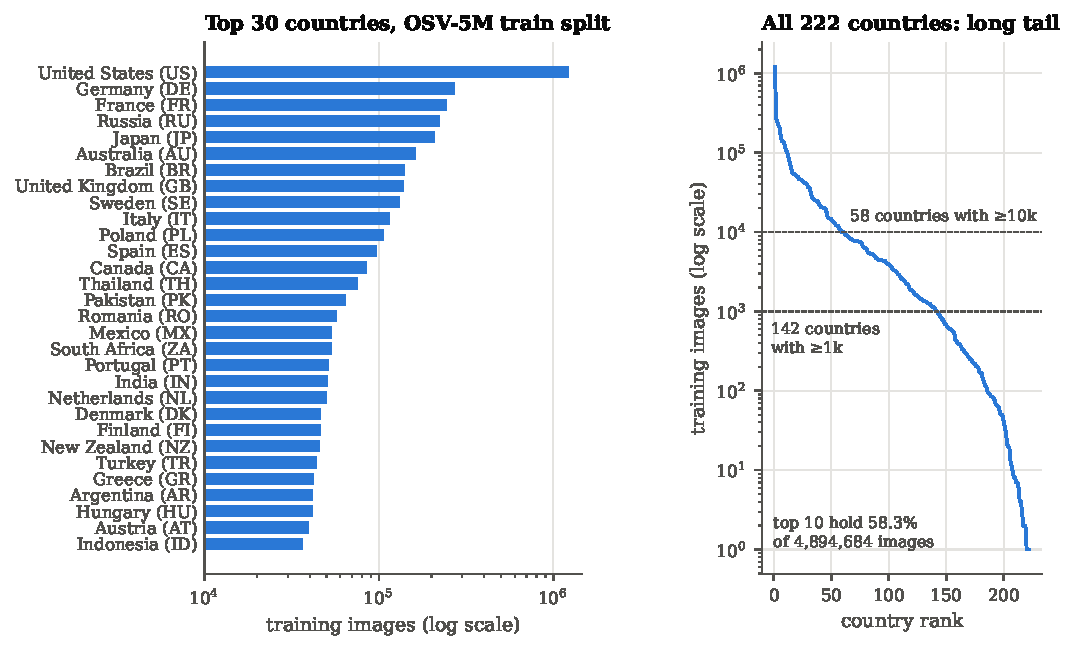
\includegraphics[width=0.78\textwidth]{fig_a_country_counts}
\caption{Country imbalance in the OSV-5M training split. Left: the 30 countries with most images (log
scale). Right: images per country for all 222 countries against their rank; the ten largest hold 58.3\% of
the 4.89M images.}
\label{fig:eda_countries}
\end{figure}

\begin{figure}[!htbp]
\centering
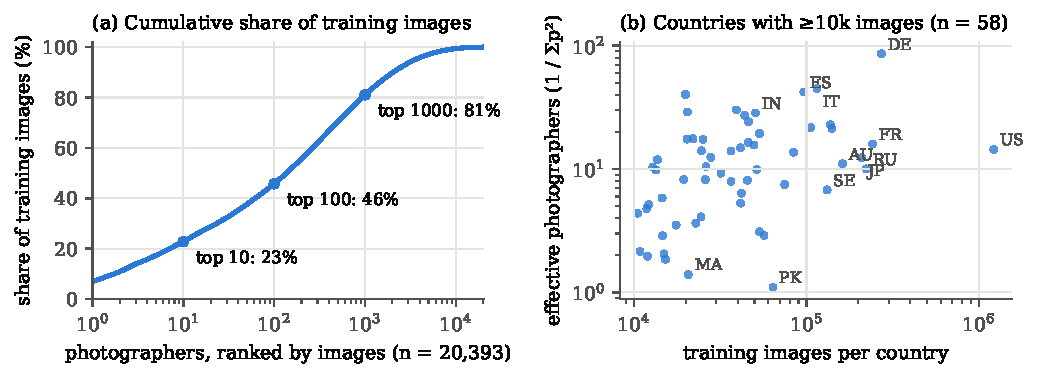
\includegraphics[width=0.85\textwidth]{fig_photographers}
\caption{Photographer concentration in the OSV-5M training split (photographers with an ID). (a)
Cumulative share of training images by photographers ranked by size: the top 100 supply 46\%. (b) For the
58 countries with at least 10{,}000 images, the effective number of photographers $1/\sum_i p_i^2$ against
the number of images: large countries are not necessarily diverse.}
\label{fig:eda_photographers}
\end{figure}

Figure~\ref{fig:samephoto} shows what a photographer's camera fingerprint looks like. Each row holds four
photos by one photographer, each from a different trip and a different road. The first photographer's
images all carry the same timestamp overlay along the bottom edge, the second's show the same white
bonnet, and the third's share a lens, mount and framing that put the horizon low and fill most of the frame
with sky. None says anything about the country, yet each is constant within a photographer and, since most photographers drive in one country, perfectly predicts the training label.

\begin{figure}[!htbp]
\centering
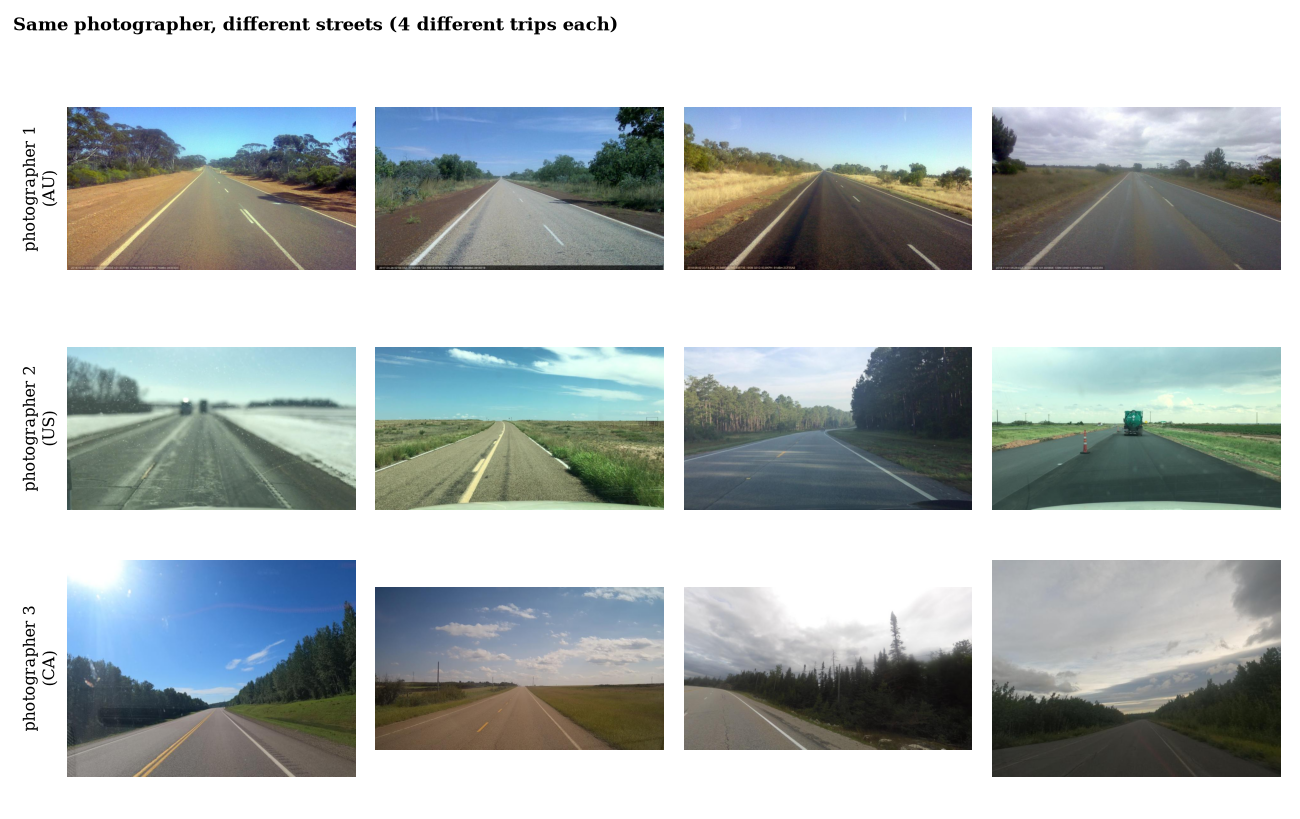
\includegraphics[width=0.7\textwidth]{fig_f_same_photographer}
\caption{The camera fingerprint: four images by each of three OSV-5M photographers (Australia, United
States, Canada), each from a different trip. Within a row the timestamp overlay, the bonnet or the framing
and colour of the camera stay the same while the roads change. Photos: OSV-5M / Mapillary photographers,
CC BY-SA 4.0.}
\label{fig:samephoto}
\end{figure}

\subsection{Subset, splits and preprocessing}
We keep the 32 countries with at least 200 photographers. Photographers are assigned 70/10/20 to
training, validation and test, stratified by each photographer's main country. Inside the training
photographers, whole groups of images linked by the same sequence or the same photographer-specific
$0.1^\circ$ cell ($\approx$11\,km) are held out as \vsh\ and \tsh: new trips and places by photographers the
model has seen. Per split and country, a fixed budget is filled by water-filling. If photographer $i$ has
$n_i$ eligible images and the budget is $B$ images, every photographer receives
\begin{equation}
\min(n_i, c^\ast)\ \text{images, where}\quad c^\ast=\max\Big\{c\in\mathbb{N}:\ \sum_i \min(n_i, c)\le B\Big\},
\end{equation}
and the few remaining slots, $B-\sum_i\min(n_i,c^\ast)$, go one each to randomly chosen photographers with
$n_i>c^\ast$. The cap $c^\ast$ is the largest one the budget allows, so the budget is spread over as many
photographers as possible and no photographer can dominate a country; within a photographer, images are taken
round-robin over its trips (Table~\ref{tab:data}).

The selection script checks that no photographer is shared between training,
validation and test and that no sequence is shared between training and any evaluation split. Images
are centre-cropped to 4:3, since the aspect ratio (4:3 or 16:9) is itself a camera property, and stored
at $128\times170$ pixels. Single images are fetched from the remote archives by HTTP range requests, so
the 139{,}696-image subset takes 1.0\,GB instead of about 245\,GB of archives.

\begin{table}[!htbp]
\centering\small
\caption{The 32-country subset. test and \tsh\ differ only in whether the photographer is in the training set.}
\label{tab:data}
\setlength{\tabcolsep}{3.5pt}\footnotesize
\begin{tabular}{@{}lrrrl@{}}
\toprule
split & images & photographers & per country & role \\
\midrule
train & 101{,}578 & 11{,}132 & 3{,}200 (ET 2{,}649, MY 2{,}929) & training \\
val & 6{,}400 & 1{,}521 & 200 & model selection, unseen photographers \\
test & 12{,}800 & 3{,}043 & 400 & \textbf{unseen photographers} \\
\vsh & 6{,}359 & 2{,}089 & $\le$200 & new trips of training photographers \\
\tsh & 12{,}559 & 3{,}037 & $\le$400 & \textbf{seen photographers, new trips} \\
extra chunks 1--3 & $+$261{,}572 & & uneven (US 60{,}637; ET, MY 0) & more data, $\le$100 per photographer \\
\bottomrule
\end{tabular}
\end{table}

\section{Methodology}
\subsection{Evaluation}
For an evaluation set with $K=32$ countries, let $T_c$ be the images of country $c$ and $\hat y_i$ the
model's prediction for image $i$ with true label $y_i$. Balanced accuracy is the mean per-class recall,
\begin{equation}
\mathrm{BA}=\frac{1}{K}\sum_{c=1}^{K}\frac{1}{|T_c|}\sum_{i\in T_c}\mathbf{1}[\hat y_i=y_i],
\end{equation}
which is $1/K\approx3.1\%$ for a random guess and equals top-1 accuracy on the balanced test set. Accuracy on
test answers the research question; the photographer gap
\begin{equation}
\Delta=\mathrm{BA}(\text{\tsh})-\mathrm{BA}(\text{test})
\end{equation}
measures how much accuracy depends on having seen the photographer.

Images by one photographer are correlated, and treating them as independent would make confidence intervals too narrow, so we use a cluster bootstrap (Field and Welsh). If an evaluation set contains $M$
photographers, one bootstrap draw samples $M$ photographers with replacement; photographer $g$ is drawn $w_g$
times, $(w_1,\dots,w_M)\sim\mathrm{Multinomial}(M;\tfrac1M,\dots,\tfrac1M)$, every image of photographer $g$
receives weight $w_g$, and BA is recomputed with these weights. Repeating this $R=1{,}000$ times gives draws
$\mathrm{BA}^{(1)},\dots,\mathrm{BA}^{(R)}$, and the 95\% confidence interval (CI) is their 2.5th to 97.5th
percentile. Test and \tsh\ have no photographers in common and are resampled independently, so the CI of
$\Delta$ comes from the differences $\mathrm{BA}^{(r)}(\text{\tsh})-\mathrm{BA}^{(r)}(\text{test})$. To
compare two models $A$ and $B$ on the same images we use \emph{paired} draws: both are scored on the same
resampled photographers, and the CI of the change comes from $d^{(r)}=\mathrm{BA}^{(r)}_B-\mathrm{BA}^{(r)}_A$.
Because $\mathrm{Var}(d)=\mathrm{Var}(\mathrm{BA}_A)+\mathrm{Var}(\mathrm{BA}_B)-2\,\mathrm{Cov}(\mathrm{BA}_A,\mathrm{BA}_B)$
and two models tend to find the same photographers easy or hard, the covariance is large and positive, so a
paired comparison detects differences far smaller than the width of either model's own interval.

Photographer splitting follows from what generalisation means here. A random split of images assumes
independent and identically distributed data, but images by one photographer share a camera, a car and a set
of roads, so such a split would put near-copies of training images in the test set. Splitting by
photographer, as grouped cross-validation does with clustered data (Roberts et al.), estimates
generalisation to new photographers, and $\Delta$ is then a generalisation gap measured between two test
distributions that differ only in whether the photographer was seen.

\subsection{Models}
All CNNs are ResNet-18 (He et al.): a $7\times7$ stem and four stages of residual blocks ending in a
512-dimensional feature (a $4\times6$ map average-pooled at our input size), dropout 0.2 and a 32-way
output layer (11.2M parameters). Images are never flipped, because mirroring swaps the driving side.
Every trained model, from the linear probe to the end-to-end network, minimises the same loss, the
multinomial cross-entropy between the predicted class probabilities (a softmax over 32 scores) and the true
country; the networks do so by stochastic gradient descent on mini-batches. The models are ordered by how many parameters are fitted to the training photographers, from none (the classical baseline only stores images and fits PCA) to all 11.2M; along this axis we expect accuracy and the risk of fitting photographer-specific detail to grow together.
\begin{enumerate}[label=(\arabic*),leftmargin=*]
\item \emph{Classical baseline} (Hays and Efros): HSV colour histogram and HOG features (Dalal and
Triggs), 2{,}268 dimensions, projected by principal component analysis (PCA) onto the 256 directions of
largest variance, since distances lose meaning in high dimensions (the curse of dimensionality), and
classified by distance-weighted 15-nearest neighbours (cosine), a non-parametric rule, on 9{,}600 training
images.
\item \emph{Linear probe}: multinomial logistic regression with an $L_2$ (ridge) penalty on frozen
ImageNet features (Deng et al.) of the same 9{,}600 images, a convex problem solved by L-BFGS: only the
linear output layer is fitted, so the representation itself cannot adapt to the training photographers.
\item \emph{Partial fine-tune}: from the probe, the last two stages and the output layer are trained on
the 101{,}578 training images on a laptop CPU (stem and stages 1--2 frozen).
\item \emph{More data}: model (3) continues on three further chunks of about 87k images each (363k
distinct images in total). The final chunk is our released checkpoint.
\item \emph{End-to-end fine-tune}: all layers of the ImageNet ResNet-18 trained on the 101{,}578
training images on a laptop GPU, \emph{once with and once without fingerprint removal}, otherwise
identical (same seed, data order and schedule).
\item \emph{$k$-NN on learned features} of (2) and (4): tests whether predictions rely on retrieving
the same photographer.
\end{enumerate}

\subsection{Removing the camera fingerprint}\label{sec:fpmethod}
The proposal planned to mask pixels that stay constant across a photographer's photos, but no pixel had
an across-photo standard deviation below 15 for any of the 60 largest photographers: bonnets reflect the
sky, photographers change cars and mounts, and the most stable regions were road, snow and sky, which are
country cues. Fingerprint removal therefore blanks the bottom 20\% of every image to the ImageNet mean
colour (blanking rather than cropping keeps the geometry fixed) and, during training, re-encodes images
as JPEG at quality 30--95 and jitters white balance ($\pm15\%$), brightness, contrast and saturation
($\pm25\%$), but not hue, since road-marking colour is a country cue. We also apply the blanking to
trained standard models \emph{at test time only}, which needs no retraining.

In terms of regularisation, fingerprint removal is data augmentation: instead of penalising the weights,
it makes the cheapest features of a photographer's camera unreliable and pushes the network towards
camera-invariant features. Like any regulariser it trades variance for bias, since every imposed
invariance also deletes whatever country information the removed pixels or colours carried.

\subsection{Training configuration}\label{sec:config}
Table~\ref{tab:config} summarises the training configuration of all models.
For the probe, raising the $L_2$ penalty from $10^{-4}$ to $10^{-2}$ lowers training accuracy from 48.7\%
to 34.3\% but raises validation accuracy from 12.8\% to 16.7\%, a clear bias--variance trade-off; the
optimum lies at the edge of the grid, so the probe slightly underestimates frozen features. For the
end-to-end runs, the training script's default (0.02 per 256, ten times more for the new output layer) overshot: the training loss rose from 3.6 to above 5 and accuracy fell to chance. A rate of 0.01 for all layers with a one-epoch warm-up, which keeps the new layer's large early gradients from disturbing the pretrained weights, trained stably. The
runs were planned for 8 epochs, but running both at once on a 16\,GB laptop made the machine swap (13--21
minutes per epoch instead of 4.5), so after epoch 4 both were resumed one after the other with the cosine
schedule shortened to 6 epochs. The learning rate therefore dropped in one step at the restart, from about
0.0062 to 0.0034; both runs went through exactly the same procedure, so their comparison stays paired.

Feasibility shaped most of these choices. The full OSV-5M archives are about 245\,GB; fetching only the selected images at $128\times170$ pixels reduced the data to 1.0\,GB, enough for a laptop. The binding constraint was compute: on a 4-core laptop CPU, ResNet-18 trains at about 10 images/s
(17 with the first stages frozen), so a 30-epoch end-to-end fine-tune on 101k images would take about 3.5
days per run, which is why models (3) and (4) froze the first layers. On a laptop GPU (Apple M5) the same
network trains at about 550 images/s, an epoch takes 4.5 minutes and an end-to-end run about half an hour.
Hyperparameters were tuned on val only: $k$ and the distance of the $k$-NN baseline, the $L_2$ penalty of
the probe, and the epoch at which each network is kept. For the CNNs we used standard fine-tuning settings
instead of a grid search, which our compute did not allow; the one change, the end-to-end learning rate,
followed a failed trial judged on the training loss. Test and \tsh\ were never used for any choice.

\begin{table}[!htbp]
\centering\small
\caption{Training configuration. val is the photographer-disjoint validation set.}
\label{tab:config}
\begin{tabularx}{\textwidth}{@{}l>{\raggedright}X>{\raggedright}X>{\raggedright}X>{\raggedright\arraybackslash}X@{}}
\toprule
 & (1) Classical / (2) Probe & (3) Partial fine-tune & (4) More data & (5) End-to-end \\
\midrule
Trained layers & -- / output layer & stages 3--4 + output & same as (3) & all \\
Training images & 9{,}600 & 101{,}578 & +87k per chunk (363k) & 101{,}578 \\
Optimiser & -- / L-BFGS & SGD, Nesterov 0.9, batch 64 & same & SGD, Nesterov 0.9, batch 256 \\
Learning rate & -- & 0.02 per 256, warm-up, cosine & 0.01 (chunk 1), 0.004 & 0.01 per 256, 1 epoch warm-up, cosine \\
Regularisation & -- / $L_2$ penalty & weight decay $10^{-4}$, dropout 0.2, label smoothing 0.1, random crops, no flips & same + class weights & same as (3) \\
Length & -- & 24 epochs of 20{,}480 & one pass per chunk & 6 epochs \\
Tuned on val & $k$, distance / $L_2\in[10^{-4},10^{-2}]$ & best epoch & best epoch & best epoch \\
Hardware, time & CPU, $\approx$7 min & 4-core CPU, 7.7\,h & CPU, $\approx$1.8\,h per chunk & Apple M5 GPU, bf16, $\approx$4.5 min per epoch (one run at a time) \\
\bottomrule
\end{tabularx}
\end{table}

\section{Results}
\subsection{Preliminary results: pilot study}
Before building the 32-country subset, we balanced the ten most frequent countries of one OSV-5M shard to
162 images each and compared photographers shared or disjoint between training and test
(Table~\ref{tab:pilot}). Both models lose close to half their accuracy once photographers are disjoint;
recall for Australia, where most images come from one photographer, drops from 81\% to 19\%. This made a
photographer-disjoint protocol the basis of our comparison.

\begin{table}[!htbp]
\centering\small
\caption{Pilot study: top-1 accuracy on ten balanced countries from one OSV-5M shard (chance 10\%; about $\pm5$ percentage points).}
\label{tab:pilot}
\begin{tabular}{@{}lcc@{}}
\toprule
Model & Photographers shared & Photographers disjoint \\
\midrule
Majority class & 9.9\% & 10.0\% \\
HSV histograms + logistic regression & 37.3\% & 19.3\% \\
Frozen ResNet-18 + logistic regression & 48.1\% & 28.1\% \\
\bottomrule
\end{tabular}
\end{table}

\subsection{Model comparison}\label{sec:comparison}
\begin{table}[!htbp]
\centering\small
\caption{Balanced accuracy (\%) on unseen (test) and seen (\tsh) photographers with 95\%
photographer-bootstrap CIs, the gap $\Delta$, top-3 accuracy on test and the median distance (km) from
misclassified test images to the predicted country. The 15-NN rows report top-1 accuracy. n/a: not computed for that model or intervention.}
\label{tab:main}
\setlength{\tabcolsep}{4pt}
\begin{tabular}{@{}llllrr@{}}
\toprule
Model & test & \tsh & $\Delta$ (pp) & top-3 & km \\
\midrule
(1) Classical & 5.6 [5.1, 6.2] & 6.5 & $+$0.9 [0.0, 1.7] & n/a & 6{,}252 \\
(2) Linear probe & 13.5 [12.8, 14.3] & 13.7 & $+$0.2 [$-$1.1, 1.4] & 29.4 & 5{,}543 \\
(3) Partial fine-tune & 28.7 [27.5, 29.8] & 34.5 & $+$5.8 [4.1, 7.5] & 51.1 & 2{,}439 \\
(4) + chunk 1 & 29.8 [28.6, 31.0] & 36.8 & $+$7.0 [5.2, 8.8] & 51.7 & 2{,}679 \\
\phantom{(4)} + chunk 2 & 30.1 [28.9, 31.3] & 37.7 & $+$7.6 [5.8, 9.4] & 51.7 & 2{,}852 \\
\phantom{(4)} + chunk 3 & 30.7 [29.4, 31.9] & 38.0 & $+$7.4 [5.6, 9.2] & 52.4 & 2{,}865 \\
\phantom{(4)} + chunk 3, bottom blanked at test & 20.9 [20.0, 21.8] & 23.9 & $+$3.0 [1.6, 4.5] & 40.0 & n/a \\
\midrule
(5) End-to-end, standard & 31.9 [30.6, 33.1] & 37.0 & $+$5.2 [3.4, 6.9] & 54.2 & 2{,}457 \\
\phantom{(5)} standard, bottom blanked at test & 22.6 [21.7, 23.5] & 25.3 & $+$2.7 [1.3, 4.2] & 42.7 & n/a \\
(5) End-to-end, fingerprint removal & 28.2 [27.1, 29.3] & 31.3 & $+$3.1 [1.3, 4.8] & 50.3 & 2{,}743 \\
\midrule
(6) 15-NN on (2) & 9.7 & 11.5 & $+$1.8 & n/a & n/a \\
(6) 15-NN on (4) & 25.3 & 32.8 & $+$7.5 & n/a & n/a \\
\bottomrule
\end{tabular}
\end{table}

Table~\ref{tab:main} and Figure~\ref{fig:scaling}a summarise the comparison. The classical baseline
reaches 5.6\% BA, less than twice chance, with errors a median 6{,}252\,km from the predicted country.
Frozen ImageNet features more than double this (13.5\%), and fine-tuning the upper network doubles it
again (28.7\%): the median error distance falls from 5{,}543 to 2{,}439\,km and top-3 accuracy rises
from 29.4\% to 51.1\%. The 15-NN classifier on the same features shows the same jump (9.7\% to 25.3\%):
fine-tuning reorganises the feature space so that images of one country lie close together.
Training all layers end to end on 101{,}578 images reaches 31.9\% on unseen photographers, $+1.2$\pp\ [0.4, 1.9] above the final partially fine-tuned model that saw 3.6 times more images, with a gap of $+5.2$\pp\ [3.4, 6.9] against $+7.4$\pp\ (paired change $-2.2$\pp\ [$-3.3$, $-1.1$]). The two models differ in more than the number of images (trainable layers, class weights, schedule and the draw of the training split), so this is an observation about the two models, not a controlled test of data quantity.

The photographer gap behaves differently. It is within 1\pp\ of zero for the classical baseline and the
probe, $+5.8$\pp\ after fine-tuning and $+7.4$\pp\ after the extra data, which added 2.0\pp\ [1.4, 2.5] on
unseen photographers but 3.5\pp\ on seen ones because it consists mostly of new trips by the same
photographers. This is the bias--variance trade-off at the level of photographers: more flexible models lower
the bias, so accuracy on new photographers rises, but they also fit regularities that hold only within the
training photographers, which is what $\Delta$ measures. The usual symptom of overfitting never appears,
since accuracy on unseen photographers keeps improving while $\Delta$ grows, so image-level validation would
not reveal the shortcut.

\begin{figure}[!htbp]
\centering
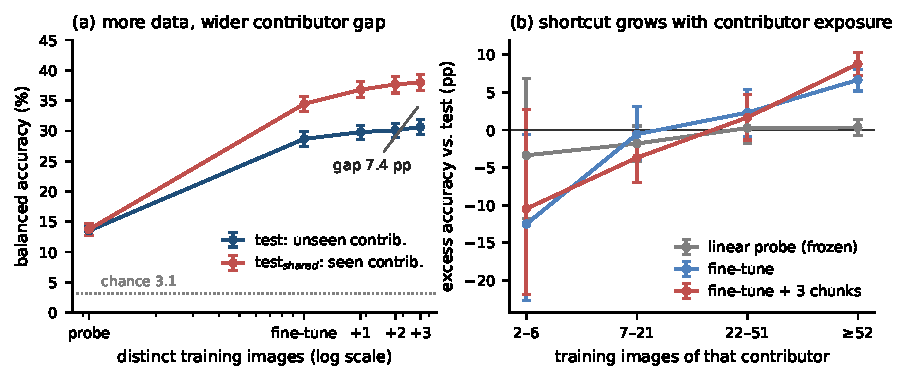
\includegraphics[width=0.85\textwidth]{scaling_decomposition}
\caption{(a) Accuracy on seen photographers (\tsh) grows faster with more training images than accuracy
on unseen ones (test). (b) Excess accuracy on new trips of seen photographers, grouped by how many of
their images were in training, with 95\% CIs. The probe stays flat, while the fine-tuned models gain up
to 8.8\pp\ for the most-seen photographers.}
\label{fig:scaling}
\end{figure}

\subsection{Which countries are hard?}\label{sec:countries}
Figure~\ref{fig:countries}a breaks accuracy down by country. For the end-to-end model, recall on unseen
photographers ranges from 9.5\% for France to 63.3\% for Ethiopia, followed by India, Taiwan and Japan
(54--58\%); the eleven hardest are ten European countries and Russia, and the ranking is stable across
models. Easy countries have no look-alike in the class set: Ethiopia is the only African country, its 400
test images come from 38 photographers with none above a 4\% share, and its precision (67\%) matches its
recall, so it is neither a memorised camera nor a default guess. Hard countries have similar neighbours:
Austria is predicted as Switzerland for 80 of its 400 images, Canada as the United States for 73, and
Belgium, Germany and Denmark as the Netherlands for 38 to 57 each.

These confusions suggest that at $128\times170$ pixels the network relies on coarse scene properties shared
within a region (vegetation, terrain, road layout) rather than on signs or plates, which are only a few
pixels large.

Against the partially fine-tuned model, end-to-end training gains most in Sweden, the United States and Germany ($+9$ to $+12$\pp) and loses most in Russia, Taiwan and Ethiopia ($-5$ to $-7$\pp). The gainers
are the countries that inverse-frequency class weights had down-weighted in the data chunks, and Ethiopia
had been up-weighted about twelve-fold, so part of the earlier model's country profile reflects its
training objective rather than the images.

\subsection{What the errors look like}\label{sec:errors}
Errors gain geographic structure as more of the network is trained (Table~\ref{tab:errors}). A random
wrong answer would stay in the true country's world region 40 to 43\% of the time; the classical baseline
is close to that, the fine-tuned networks reach 59 to 62\%. Driving side is the clearest learned cue: images
from the seven left-hand-traffic countries go to a left-hand-traffic country 32\% of the time for the
classical baseline but 68 to 70\% for every fine-tuned model, against 22\% for a uniform guess, which is why
we never flip images.

\begin{table}[!htbp]
\centering\small
\caption{Structure of the errors on test (unseen photographers). ``Same region'': share of misclassified
images whose predicted country lies in the same world region as the true one; chance assumes a uniform
wrong answer. ``Left $\to$ left'': share of images from left-hand-traffic countries assigned to a
left-hand-traffic country (uniform guess 22\%).}
\label{tab:errors}
\begin{tabular}{@{}lrrrr@{}}
\toprule
Model & error rate & same region (chance) & left $\to$ left & median error (km) \\
\midrule
(1) Classical & 94.4\% & 44.4\% (39.7\%) & 32.4\% & 6{,}252 \\
(2) Linear probe & 86.5\% & 47.8\% (41.0\%) & 43.3\% & 5{,}543 \\
(4) Partial fine-tune + 3 chunks & 69.3\% & 59.1\% (42.8\%) & 68.4\% & 2{,}865 \\
(5) End-to-end, standard & 68.1\% & 62.1\% (42.6\%) & 70.3\% & 2{,}457 \\
(5) End-to-end, fingerprint removal & 71.8\% & 59.1\% (42.5\%) & 69.6\% & 2{,}743 \\
\bottomrule
\end{tabular}
\end{table}

\begin{figure}[!htbp]
\centering
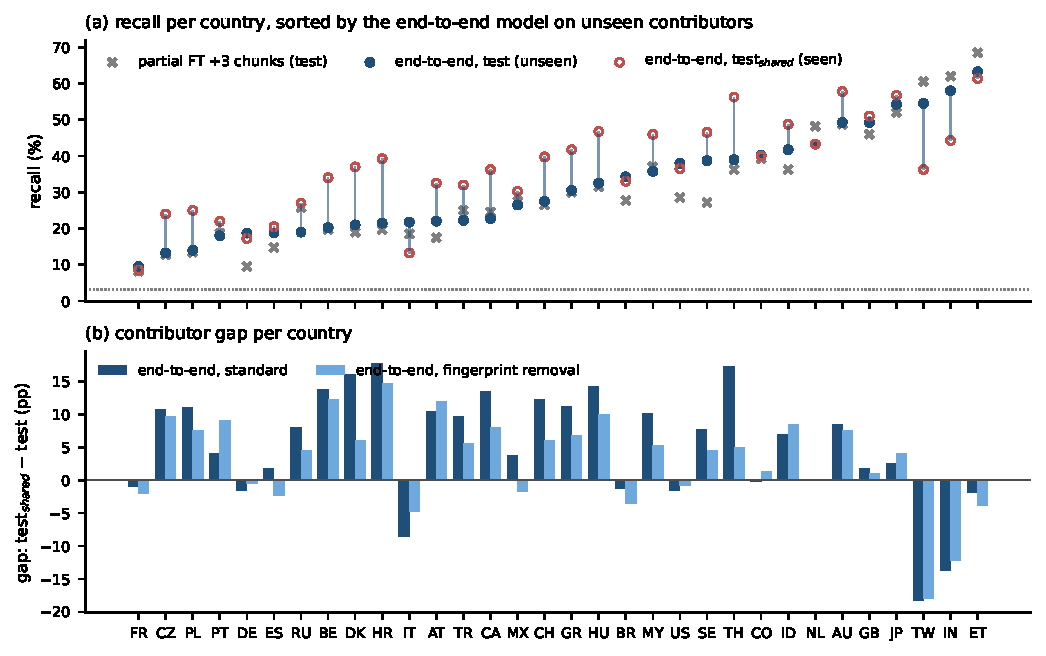
\includegraphics[width=0.9\textwidth]{fig_countries}
\caption{(a) Recall per country (ISO codes), sorted by the end-to-end model's recall on unseen
photographers (filled); lines connect it with recall on seen photographers (open); crosses show the final
partially fine-tuned model. (b) Per-country photographer gap of the end-to-end model without and with
fingerprint removal. With 400 test images per country (272--400 in \tsh), each value carries roughly
$\pm4$--5\pp\ of sampling uncertainty.}
\label{fig:countries}
\end{figure}

\section{Where the photographer gap comes from}\label{sec:gap}
\subsection{Exposure}
If seen photographers simply photographed easier places, accuracy on their new trips would not depend on
how many of their images were in training. We group \tsh\ photographers by their number of training images
and compute the excess accuracy
\begin{equation}
E_B=\frac{1}{|B|}\sum_{i\in B}\big(\mathbf{1}[\hat y_i=y_i]-a_{c(i)}\big),
\end{equation}
where $a_c$ is the model's accuracy on country $c$ in test, so each image is compared with its own
country's level for unseen photographers. For the probe, $E_B$ is flat ($+0.3$\pp\ [$-0.7$, 1.4] at 52 or
more images); for the final partially fine-tuned model it reaches $+8.8$\pp\ [7.3, 10.3]
(Figure~\ref{fig:scaling}b). The end-to-end model shows the same dose--response on its own training counts
(Figure~\ref{fig:exposure}): from $-3.7$\pp\ [$-6.2$, $-1.2$] for photographers with 2--5 training images to
$+8.9$\pp\ [6.8, 10.8] for those with more than 25, who supply 56\% of \tsh. The frozen probe, scored on
the same images, rules out that heavily represented photographers simply take easier photos: its curve
is flat. With
fingerprint removal the curve keeps its shape but is lower throughout ($+6.3$\pp\ [4.3, 8.1] in the top
bin): memorisation is weakened, not removed.

\begin{figure}[!htbp]
\centering
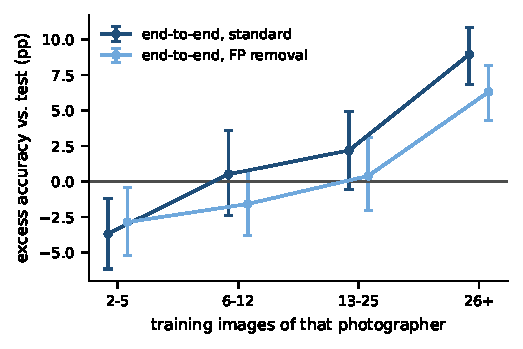
\includegraphics[width=0.55\textwidth]{fig_exposure}
\caption{Exposure dose--response of the end-to-end models: excess accuracy on new trips of seen
photographers, relative to the same countries' accuracy on unseen photographers, by the photographer's number
of training images; 95\% photographer-bootstrap CIs.}
\label{fig:exposure}
\end{figure}

\subsection{Place or camera?}\label{sec:place}
Held-out trips exclude the same sequence and 11\,km cell, but a new trip can still be near roads the photographer drove in training, so the gap could reflect familiar places as well as a familiar camera. We therefore measure, for each \tsh\ image, the distance to the nearest training image by the same
photographer, and compute the excess accuracy $E_B$ in distance bins, keeping only trips in a country where
the photographer also has training images (95\% of \tsh). Table~\ref{tab:place} shows that the advantage is
local: $+8.0$\pp\ within 25\,km, which covers 62\% of \tsh, $+3.7$\pp\ at 25--100\,km and none at
100--500\,km; the 197 images at 500\,km or more are even below the unseen-photographer level, plausibly
because the model expects a photographer's region of the country. Fingerprint removal lowers the curve by
1.7 to 2.6\pp\ in every bin up to 500\,km. Since $E_B$ is measured against each model's own accuracy
on unseen photographers, this shift is not a general accuracy loss. We read the gap as two parts: a local
part that fades with distance, where the model recognises the places a photographer drives together with
their camera, and a camera part of about 2\pp\ that fingerprint removal removes. Because heavily exposed
photographers also have more training images near their new trips, distance and exposure are correlated,
and this analysis does not fully separate them.

\begin{table}[!htbp]
\centering\small
\caption{Place or camera: excess accuracy (pp) on new trips of seen photographers by distance to the same
photographer's nearest training image, for trips in a country where the photographer has training images;
95\% photographer-clustered bootstrap CIs.}
\label{tab:place}
\begin{tabular}{@{}lrrll@{}}
\toprule
distance & images & photographers & end-to-end & + fingerprint removal \\
\midrule
$<25$\,km & 7{,}812 & 2{,}164 & $+8.0$ [6.4, 9.8] & $+5.4$ [3.8, 7.0] \\
25--100\,km & 2{,}924 & 1{,}188 & $+3.7$ [1.2, 6.2] & $+2.0$ [$-0.3$, 4.2] \\
100--500\,km & 1{,}020 & 553 & $+0.3$ [$-2.9$, 3.7] & $-2.0$ [$-5.3$, 1.4] \\
$\geq500$\,km & 197 & 125 & $-10.2$ [$-16.4$, $-3.8$] & $-8.7$ [$-14.7$, $-2.3$] \\
\bottomrule
\end{tabular}
\end{table}

\subsection{Retrieval}
With 1-NN on the final partially fine-tuned features, 6.9\% of \tsh\ images have a photo by the same
photographer as their nearest neighbour in \vsh. These are 90.6\% correct against 22.0\% for the rest, which
accounts for about 4.7\pp\ of the 1-NN classifier's 6.7\pp\ gap. The end-to-end model behaves alike (6.3\% of
queries, 91.2\% against 21.2\% correct). Fingerprint removal lowers the share of same-photographer neighbours
to 3.9\%: the mechanism is unchanged, it simply fires less often.

\subsection{Photographer verification}
The proposed photographer classifier cannot be trained, since held-out photographers have at most four
training images, so we ask instead whether images by the same photographer from different trips are more
similar (cosine) than images by different photographers from the same country. The area under the ROC
curve (0.5 is chance) is 0.59--0.62 for frozen features, 0.57 for both fine-tuned models and 0.55--0.56 with
fingerprint removal, whose features also have fewer same-photographer nearest neighbours (9.5\% against
14.0\% on test; random pairs 0.1\%). Photographer style is weakly but consistently visible in every
representation, most in the frozen one, yet only a classifier fitted to the training photographers turns
it into a gap.

\subsection{Where in the image}\label{sec:gradcam}
Grad-CAM (Selvaraju et al.) on the last stage shows where the evidence for the predicted class lies
(Figure~\ref{fig:gradcam}). On 1{,}600 images, both the partially and the end-to-end fine-tuned model put
about 20\% of their evidence in the bottom 20\% of the frame, exactly its share of the area, and the maps
point to vegetation, buildings, poles and road edges rather than to the bonnet. The $4\times6$ map is
coarse, so these region shares are indicative rather than a precise localisation. Grad-CAM also locates the
evidence for the \emph{country}, not for the photographer, so this is consistent with the band mattering
mainly for photographers the model has seen, which the blanking experiments below confirm.

\begin{figure}[!htbp]
\centering
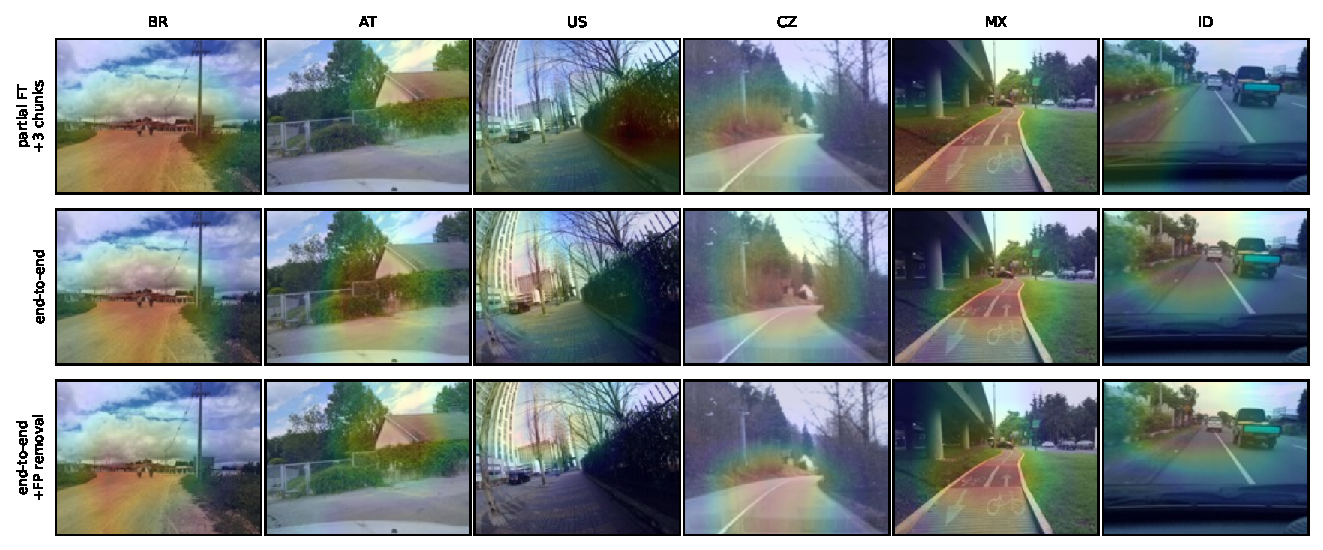
\includegraphics[width=\textwidth]{gradcam_panel}
\caption{Grad-CAM maps of the predicted class for test-set images (country codes above). Photos:
OSV-5M / Mapillary photographers, CC BY-SA 4.0.}
\label{fig:gradcam}
\end{figure}

\section{Removing the camera fingerprint}\label{sec:fp}
\subsection{At test time}
Blanking the bottom 20\% of every evaluation image without retraining lowers the final partially
fine-tuned model's BA from 30.7\% to 20.9\% on unseen and from 38.0\% to 23.9\% on seen photographers: a paired
change of $-9.8$\pp\ [$-10.8$, $-8.8$] in test BA and $-4.3$\pp\ [$-5.8$, $-2.9$] in the gap, which falls to
$+3.0$\pp. For the end-to-end model the changes are $-9.2$\pp\ and $-2.4$\pp\ (gap $+2.7$\pp). The band holds roughly half of each gap but a third of the accuracy, so both models read the bonnet and dashboard disproportionately for familiar photographers; part of the loss, however, is distribution shift, since neither model saw a blanked image in training.

\subsection{During training}
Trained with fingerprint removal, the end-to-end model reaches 28.2\% on unseen and 31.3\% on seen
photographers, against 31.9\% and 37.0\% without it (Table~\ref{tab:main}, Figure~\ref{fig:e2e}). Paired,
test BA changes by $-3.6$\pp\ [$-4.5$, $-2.8$], \tsh\ BA by $-5.7$\pp\ [$-6.6$, $-4.9$] and the gap by
$-2.1$\pp\ [$-3.3$, $-0.9$], from $+5.2$ to $+3.1$\pp. Seen photographers lose more than unseen ones, the
signature of a shortcut being removed, and the validation gap during training opens to only $+1.8$\pp\
instead of $+3.9$\pp.

Per country (Figure~\ref{fig:countries}b), the gap shrinks in 21 of 32 countries, most where it was
largest (Thailand $-12$\pp, Denmark $-10$\pp), but the per-country gaps of the two models stay highly
correlated ($r=0.91$): fingerprint removal scales the shortcut down rather than moving it. The accuracy
cost falls on countries such as Switzerland, Thailand and Mexico ($-7$ to $-8$\pp), because the bottom of
the frame shows road surface and markings, which are genuine country cues. Taiwan and India have strongly negative gaps under both models, plausibly because a few heavy photographers gave a narrow view of those countries; with 400 images per country this is a hypothesis.

\begin{figure}[!htbp]
\centering
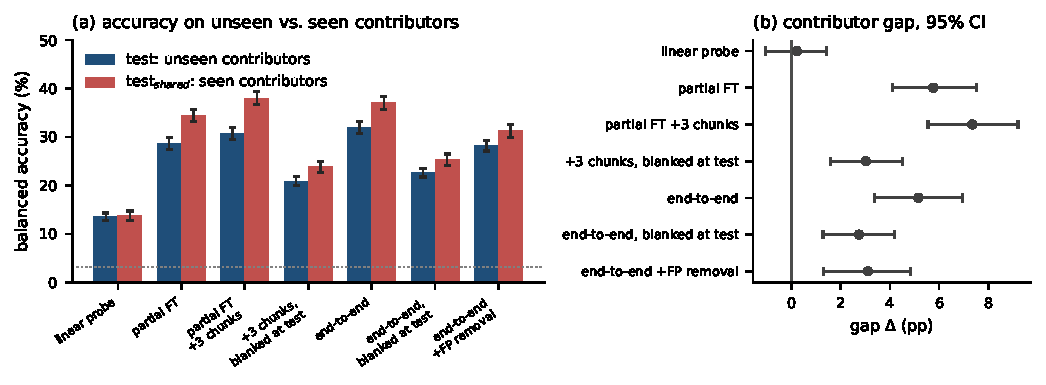
\includegraphics[width=0.88\textwidth]{fig_e2e}\\[2pt]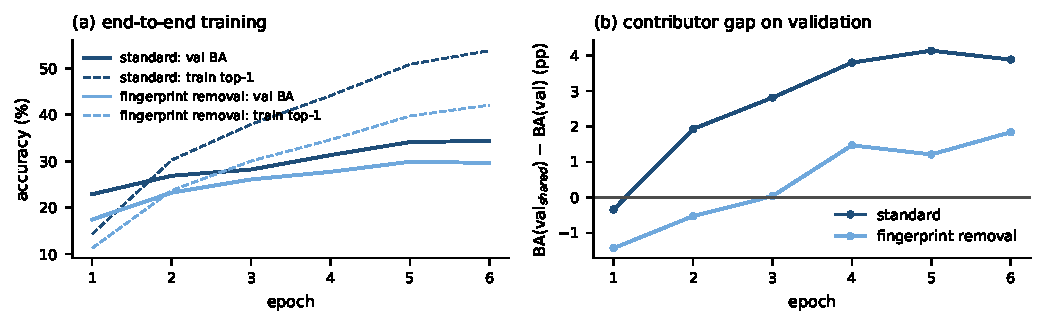
\includegraphics[width=0.88\textwidth]{fig_curves}
\caption{Top: balanced accuracy on unseen and seen photographers and the photographer gap with 95\% CIs (E2E: end-to-end; blank: bottom 20\% blanked at test time; +FP: trained with fingerprint removal), for
all models and interventions. Bottom: end-to-end training curves without and with fingerprint removal.}
\label{fig:e2e}
\end{figure}

\subsection{Combining the frames of a trip}\label{sec:trips}
Averaging log-probabilities over the frames of a trip barely changes overall accuracy, because most trips
in our test set have a single frame (10{,}658 trips for 12{,}800 images). On the 1{,}126 test trips with two
or more frames, however, it lifts the end-to-end model from 33.9\% to 40.7\%: a few frames of one trip add
about 7\pp, more than tripling the training data did. It also amplifies the photographer gap on those trips, from 3.0 to 7.0\pp\ (1.2 to 3.8\pp\ with fingerprint removal), since frames of one trip share the camera, so their votes compound photographer as well as country evidence.

\section{Discussion}
\subsection{Countries are learned}
On photographers it has never seen, the end-to-end ResNet-18 is right on 31.9\% of images over 32
countries, ten times chance, and its errors respect driving side and world region. These are country cues, not camera cues, because they hold for unseen photographers, and most come from adapting the network to street scenes: colour and gradient statistics give 5.6\%, frozen ImageNet features 13.5\%.

\subsection{Photographers are learned too}
The same network is 5.2\pp\ more accurate on new trips of photographers it was trained on (7.4\pp\ for the
model that saw more images of them). The gap is absent from frozen features, rises with a photographer's
training images, is carried mostly by same-photographer retrieval, and shrinks when camera cues are
removed, so it lies in the photographers rather than in geography in general; the distance analysis shows
that it is concentrated near the places they drove in training, where a familiar camera and familiar roads
combine (Section~\ref{sec:place}). Minimising the training cross-entropy rewards any feature correlated with the label, and gradient descent cannot tell geography from who happened to drive there: a camera that only ever
drives in Thailand is a perfect, cheap feature for ``Thailand''. The photographer is a confounder of the
image--country relation, the classic setting for shortcut learning (Geirhos et al.).

\subsection{More of the same data is not the cure}
The extra 261k images mostly repeat photographers already in training; they bought 2.0\pp\ on unseen but
3.5\pp\ on seen photographers, and the end-to-end model trained on 101k images did at least as well on
unseen photographers with a smaller gap. Images by one photographer are not independent: a hundred more add little about the country but much about the photographer, so the effective sample size is closer to the number of photographers than of images. This is why the United
States, with 1.2M training images but an effective number of photographers of 14, is not an easy class, and
why the number of distinct photographers per country is the quantity worth growing.

\subsection{Removing the camera has a price}
Fingerprint removal cuts the gap by about 40\% but costs 3.6\pp\ on new photographers: the bias--variance
trade-off in its plainest form, because camera and country share pixels. The surviving gap and dose--response show photographer cues elsewhere too (windscreen reflections, mounts, lens, horizon height, habitual roads and seasons), some entangled with geography itself.
For the best accuracy on new photographers the standard model is better; for accuracy independent of who took the photo, fingerprint removal is, and it must be applied during training: blanking at test time reaches a similar gap at two and a half times the cost.

\subsection{Implications for benchmarks}
On the official OSV-5M split, 98.2\% of test images come from training photographers, so published
accuracies, including the 68.0\% of a fine-tuned ViT-L/14 (Astruc et al.), mix country and photographer
recognition. For our ResNet-18 the photographer share is worth several points. For larger models it could
go either way: the gap grew with images per photographer, which larger models trained on all 4.9M images
see in abundance, but at higher resolution signs, plates and text become legible, which could reduce
reliance on the camera. We cannot measure this here, but it argues for reporting photographer-disjoint accuracy alongside the official one.

\subsection{Limitations}\label{sec:limits}
All runs use one seed and one split, and the CIs ignore model selection and training randomness, so the
2.1\pp\ effect of fingerprint removal rests on a single pair of training runs. The per-country, exposure
and trip analyses reuse the same test sets many times and are exploratory, without correction for multiple
comparisons. The end-to-end models were
trained for only 6 epochs with a schedule shortened after epoch 4, and the from-scratch pair of the planned
$2\times2$ design and the probe refit were not run; the proposed static-pixel masks and photographer
classifier were replaced by bottom-band blanking and pairwise verification. At $128\times170$ pixels
absolute accuracies are lower bounds, while $\Delta$, which compares two test sets through one model, is
less affected. Fingerprint removal changes three things at once and misses windscreen reflections, mounts
and colour profiles. Country labels come from GPS positions, and OSV-5M's driving-side field marks the
United Kingdom as right-hand traffic, so we used real-world driving sides. Finally, the subset script is not
bit-reproducible across platforms, so the end-to-end training set is a statistically equivalent re-draw
that keeps the original evaluation images and excludes every held-out trip; the released checkpoint
reproduces all 38{,}118 committed predictions exactly on the new machine.

\section{Ethical considerations}
\subsection{Photographer identification}
Our central finding is also a privacy risk. The features place two photos by the same photographer next to
each other 10 to 16\% of the time against 0.1\% by chance, even for photographers never seen in training,
so they could link anonymous uploads to one person or vehicle and, with GPS metadata, reconstruct where someone drives. This is camera identification (Luk\'a\v{s} et al.) learned implicitly, so geolocation models should be checked for photographer leakage, and fingerprint removal doubles as a privacy measure.

\subsection{Geolocation and data}
The same methods scale towards street-level geolocation (Haas et al.), which can expose where people live
or travel. OSV-5M is CC BY-SA with faces and licence plates blurred by Mapillary; we use it for research
only, show a few attributed examples and redistribute no images. The data are also geographically unbalanced: requiring 200 photographers leaves out almost all of Africa and much of Asia and Latin America, so such accuracy describes well-mapped countries, and such models serve under-mapped regions worst.

\section{Future work}
The first step is to complete the planned $2\times2$ design and repeat each condition with several seeds,
so that the effect of fingerprint removal comes with an uncertainty over training runs; a network trained
from scratch, without ImageNet features to fall back on, should lean more on the camera. Beyond
hand-designed fingerprint removal, an adversarial photographer classifier trained through gradient reversal
(Ganin et al.) could remove photographer information from the features wherever it comes from, and
per-photographer reweighting or a group-robust objective (Sagawa et al.) could stop heavy photographers from
dominating the fit; our verification AUC and exposure analysis are ready-made measures of success. Training on whole trips and at higher resolution, where signs become legible, should raise accuracy, and a photographer-disjoint re-split of the OSV-5M test set would let others measure the photographer advantage of larger models.

\section{Conclusion}
A ResNet-18 trained on crowd-sourced street views learns country cues that transfer to photographers it
has never seen: 31.9\% balanced accuracy over 32 countries after end-to-end fine-tuning, against 3.1\%
chance and 13.5\% for frozen ImageNet features, with errors that respect driving side and world region.
But part of what it learns is the photographers themselves: a photographer gap of $+5.2$\pp\ ($+7.4$\pp\
after more images of the same photographers) that frozen features do not show, that rises with a
photographer's exposure, and that retrieval of the same photographer explains. The gap is local: it is
largest on trips near the photographer's training trips and absent beyond 100\,km, so it combines familiar
places with a familiar camera. Training with fingerprint removal lowers it by about 2\pp\ at every distance up to 500\,km,
to $+3.1$\pp\ overall, at a cost of 3.6\pp\ on new photographers. Photographer-disjoint evaluation, and more
photographers rather than more images per photographer, should be the default for geolocation models built
from crowd-sourced data. In the class game, \emph{Dashcam Duel}, players compete against the partially
fine-tuned model, which gets 31\% of its 640 test photos right. Code and run
artefacts: \url{https://github.com/LaGuadana/country-not-camera}.

\section*{Works cited}
\begin{description}[leftmargin=2em,labelindent=0pt,font=\normalfont,itemsep=2pt]\small
\item Astruc, Guillaume, et al. ``OpenStreetView-5M: The Many Roads to Global Visual Geolocation.'' \emph{Proceedings of the IEEE/CVF Conference on Computer Vision and Pattern Recognition}, 2024, pp. 21967--77, https://doi.org/10.1109/CVPR52733.2024.02074.
\item Dalal, Navneet, and Bill Triggs. ``Histograms of Oriented Gradients for Human Detection.'' \emph{Proceedings of the IEEE Conference on Computer Vision and Pattern Recognition}, vol. 1, 2005, pp. 886--93.
\item Deng, Jia, et al. ``ImageNet: A Large-Scale Hierarchical Image Database.'' \emph{Proceedings of the IEEE Conference on Computer Vision and Pattern Recognition}, 2009, pp. 248--55.
\item Doersch, Carl, et al. ``What Makes Paris Look like Paris?'' \emph{ACM Transactions on Graphics}, vol. 31, no. 4, 2012, article 101.
\item Field, Christopher A., and Alan H. Welsh. ``Bootstrapping Clustered Data.'' \emph{Journal of the Royal Statistical Society: Series B (Statistical Methodology)}, vol. 69, no. 3, 2007, pp. 369--90.
\item Ganin, Yaroslav, et al. ``Domain-Adversarial Training of Neural Networks.'' \emph{Journal of Machine Learning Research}, vol. 17, no. 59, 2016, pp. 1--35.
\item Geirhos, Robert, et al. ``Shortcut Learning in Deep Neural Networks.'' \emph{Nature Machine Intelligence}, vol. 2, no. 11, 2020, pp. 665--73.
\item \emph{GeoGuessr}. GeoGuessr AB, www.geoguessr.com. Accessed 11 Oct. 2026.
\item Haas, Lukas, et al. ``PIGEON: Predicting Image Geolocations.'' \emph{Proceedings of the IEEE/CVF Conference on Computer Vision and Pattern Recognition}, 2024.
\item Hays, James, and Alexei A. Efros. ``IM2GPS: Estimating Geographic Information from a Single Image.'' \emph{Proceedings of the IEEE Conference on Computer Vision and Pattern Recognition}, 2008, pp. 1--8.
\item He, Kaiming, et al. ``Deep Residual Learning for Image Recognition.'' \emph{Proceedings of the IEEE Conference on Computer Vision and Pattern Recognition}, 2016, pp. 770--78.
\item Kaufman, Shachar, et al. ``Leakage in Data Mining: Formulation, Detection, and Avoidance.'' \emph{ACM Transactions on Knowledge Discovery from Data}, vol. 6, no. 4, 2012, article 15.
\item Luk\'a\v{s}, Jan, et al. ``Digital Camera Identification from Sensor Pattern Noise.'' \emph{IEEE Transactions on Information Forensics and Security}, vol. 1, no. 2, 2006, pp. 205--14.
\item Roberts, David R., et al. ``Cross-Validation Strategies for Data with Temporal, Spatial, Hierarchical, or Phylogenetic Structure.'' \emph{Ecography}, vol. 40, no. 8, 2017, pp. 913--29.
\item Sagawa, Shiori, et al. ``Distributionally Robust Neural Networks for Group Shifts: On the Importance of Regularization for Worst-Case Generalization.'' \emph{International Conference on Learning Representations}, 2020.
\item Selvaraju, Ramprasaath R., et al. ``Grad-CAM: Visual Explanations from Deep Networks via Gradient-Based Localization.'' \emph{Proceedings of the IEEE International Conference on Computer Vision}, 2017, pp. 618--26.
\item Torralba, Antonio, and Alexei A. Efros. ``Unbiased Look at Dataset Bias.'' \emph{Proceedings of the IEEE Conference on Computer Vision and Pattern Recognition}, 2011, pp. 1521--28.
\item Vivanco Cepeda, Vicente, et al. ``GeoCLIP: Clip-Inspired Alignment between Locations and Images for Effective Worldwide Geo-Localization.'' \emph{Advances in Neural Information Processing Systems}, vol. 36, 2023.
\item Vo, Nam, Nathan Jacobs, and James Hays. ``Revisiting IM2GPS in the Deep Learning Era.'' \emph{Proceedings of the IEEE International Conference on Computer Vision}, 2017.
\item Weyand, Tobias, et al. ``PlaNet: Photo Geolocation with Convolutional Neural Networks.'' \emph{Proceedings of the European Conference on Computer Vision}, 2016.
\item Zech, John R., et al. ``Variable Generalization Performance of a Deep Learning Model to Detect Pneumonia in Chest Radiographs: A Cross-Sectional Study.'' \emph{PLOS Medicine}, vol. 15, no. 11, 2018, e1002683.
\end{description}

\section*{AI acknowledgement}
In line with the course policy on AI use, and as announced in our progress report, we disclose how
generative AI (Claude models by Anthropic, used through the Claude Code assistant) was used in this project.

\subsection*{What the AI did}
\begin{itemize}[leftmargin=*]
\item \emph{Code.} Part of the code in the repository was written and debugged by the AI under our direction: the data
pipeline (subset selection, range-request download, image packing), the training and evaluation scripts,
the analysis scripts (photographer probe, retrieval, exposure, error geography, Grad-CAM, trip aggregation,
per-country and error-structure analyses) and the figure scripts. Commits it co-authored are marked as such
in the repository history.
\item \emph{Experiments.} In the final phase it ran the end-to-end experiments on our devices: it adapted the
code to the laptop GPU, rebuilt the dataset on the new machine, chose the replacement learning rate after
the default collapsed in a trial, changed the schedule when the concurrent runs made the machine swap
(Section~\ref{sec:config}), and ran the test-time blanking, Grad-CAM, trip, per-country and error-structure
analyses.
\item \emph{Writing.} We drafted the text and the main concepts of the proposal, the progress report and this
report; the AI finalised them, editing wording and structure, assisting in the results sections and
discussion from our inputs, and producing the tables and figures.
\end{itemize}

\subsection*{What we did}
We chose the research question, the dataset and the photographer-disjoint
evaluation design, defined the main concepts of the analysis, drafted the reports, decided which
experiments to run and which to drop under our time budget, and reviewed, edited and take responsibility
for all code, results and text.

\subsection*{How outputs were checked}
Every number in this report is produced by a script in the
repository and stored in a results or metrics file next to the run that produced it; we checked reported
numbers against those files. The released checkpoint was re-evaluated on a second machine, which
reproduced all 38{,}118 committed predictions exactly. Interpretations the AI proposed that our data cannot
establish are stated as hypotheses (for example the negative gaps of Taiwan and India).
\end{document}
